% !TEX root = ../../I4PRJ, Grp3 - Rapport.tex
\chapter{Specifikation og Analyse}\label{SpecOgAnalyse}
Afsnittet beskriver specifikations- og analysearbejdet. Specifikationsarbejdet begyndte med analyse af projektformulering. Analysen bestod af at løse de problemstillinger, som projektformuleringen rejser vha. user stories. User stories, som er resultatet af analyse arbejdet, ses i det tidligere afsnit~\ref{FunkKrav}. Gruppen bestemte at have fokus på at lave de dele, som har mest værdig for slutbrugeren af systemet. User stories blev prioriteret ved en MoSCoW analyse, som også fremgår i tabel~\ref{table:functional}. Til at danne overblik over systemets domæner, foretog gruppen en domæneanalyse\todo{ref til metoden domæneanalyse, som ikke findes} af user stories. Resultatet af analysen ses på figur~\ref{fig:domainmodelboundary}.

\begin{figure}
	\centering
	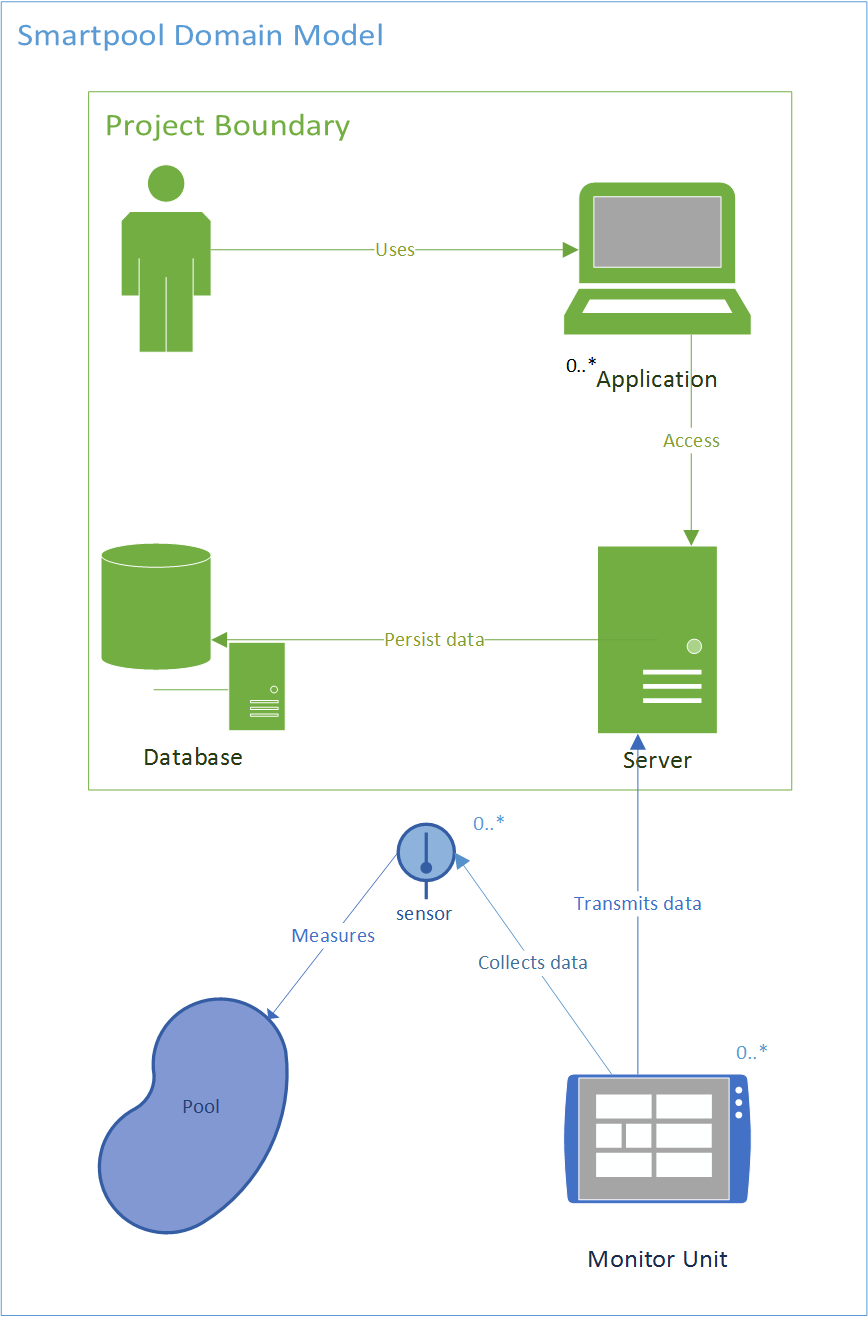
\includegraphics[width=0.7\linewidth]{figs/ProjectBoundary}
	\caption{Domænemodel for systemet}
	\label{fig:domainmodelboundary}
\end{figure}

Smartpool projektet afgrænses til at være foruden dataopsamlingsdelen, hvilket også er vist i Figur~\ref{fig:domainmodelboundary}. Dette vises med en grøn markering af de dele projektet kommer til at indeholde.

For en domænebeskrivelse se dokumentationen afsnit Domænebeskrivelser under Kravspecifikation.

Specifikations- og analysearbejde er ligesom alt andet i projektet en iterativproces. Det betyder, at de user stories som er defineret i denne rapport, ikke nødvendigvis er de samme, som da udviklingsprocessen startede. Undervejs i denne proces kan såvel domæneanalysen og -modellen have ændret sig. I samme proces er kvalitetskravene for systemet blevet bestemt, ved løbende at analysere givne problemstillingerne vha. FURPS. Resultatet af denne proces ses i \todo{ref kravafsnittet} 